% TRACE-rPPG extended abstract, NSysS 2026 poster track.
% Generated by scripts/build_deliverables.py from results files; edit the
% template (template_abstract.tex), not this output. Compile on Overleaf
% with the IEEEtran class; figures are in ./figures.
\documentclass[conference]{IEEEtran}
\usepackage{graphicx}
\usepackage{booktabs}
\usepackage{amsmath}
\usepackage{url}

\begin{document}

\title{Does Video Compression Widen the Skin-Tone Gap in Remote Photoplethysmography? A Simulated Pilot and a Classical Mitigation}

\author{\IEEEauthorblockN{Ahammad Shawki \and S. M. Abu Fayeem}
\IEEEauthorblockA{[Department, University], Dhaka, Bangladesh\\
[emails]}}

\maketitle

\begin{abstract}
Remote photoplethysmography (rPPG) estimates heart rate from the colour change each heartbeat causes in facial skin. It is known to be less accurate on darker skin, and separately known to degrade under video compression, but the interaction has not been measured. Because bitrate is a network-layer decision, an interaction would mean that constrained connections compound a demographic disadvantage. We build a fully classical pipeline (convolution filtering, Fourier spectra, no learned estimator), a compression harness with lossless controls, and a face-video simulator with controllable melanin, and run a pilot of {{N_SUBJECTS}} simulated volunteers across {{CODECS}} at {{BITRATES}} kbps. {{HEADLINE}} We also evaluate TRACE, a signal-quality-adaptive fusion of classical methods with a pulse-blind artifact reference, and two pretrained neural baselines. All results are simulated; the protocol for recorded participants is ready.
\end{abstract}

\section{Motivation and Gap}
Chrominance rPPG methods degrade on Fitzpatrick V to VI skin \cite{dasari2021,nowara2020}, and compression measurably damages rPPG \cite{mcduff2017,nowara2019}. The field names both factors as separately studied. An OpenAlex search (2,023 rPPG papers; 51 on compression, 121 on skin tone) found 3 papers mentioning both and none measuring the interaction. Melanin absorbs more light, so the pulse is a smaller change in pixel levels on darker skin; codecs subsample chroma and quantise small temporal changes. A weaker signal should cross the codec noise floor at a higher bitrate, making the disparity multiplicative rather than additive.

\section{Method}
\textbf{Pipeline.} Haar face detection with phase-correlation tracking (the Fourier shift theorem; re-detecting every few frames made the box wobble enough to destroy the pulse on dark skin); forehead and cheek means with an adaptive chroma mask; moving-average detrending and a hand-built windowed-sinc bandpass (0.7 to 4 Hz), both convolutions; green, CHROM \cite{dehaan2013} and POS \cite{wang2017}; a windowed FFT with parabolic peak interpolation and a sub-harmonic check.

\textbf{TRACE.} Each method is scored by the fraction of in-band spectral power at its peak and harmonic. Scores alone failed on held-out data (periodic motion is also a concentrated peak), so a pulse-blind artifact reference was added: normalised RGB along the brightness direction with a nominal pulse direction removed. Its spectrum masks each method's spectrum ($(1-A(f))^{k}$, $k={{MASK_K}}$) and penalises a method whose peak coincides with artifact power; spectra are fused with weights $q^{\gamma}$, $\gamma={{GAMMA}}$, and a reading below quality {{CONF}} is reported as low confidence. Parameters were tuned on 48 simulated subjects and frozen before testing.

\textbf{Simulator and harness.} A public-domain portrait is rendered at 640x480, 30 fps with a two-layer reflectance model: melanin attenuates light with wavelength-dependent absorption, surface reflection is channel neutral, plus motion, lighting drift, chromatic screen light and sensor noise, and a heartbeat with known beat times. Codecs, detector and pipeline are real. Every condition re-encodes the same lossless source; controls separate colour conversion (YUV 4:4:4), chroma subsampling (4:2:0) and quantisation. The lossless control decodes bit-identically.

\textbf{Statistics.} Per-subject, per-condition MAE is modelled as $\text{err} \sim \log_2(\text{kbps}) \times \text{dark} + (1 \mid \text{subject})$; the interaction coefficient, with Wald and subject-bootstrap intervals, is the claim.

\section{Results (simulated)}
\begin{figure}[t]
\centering
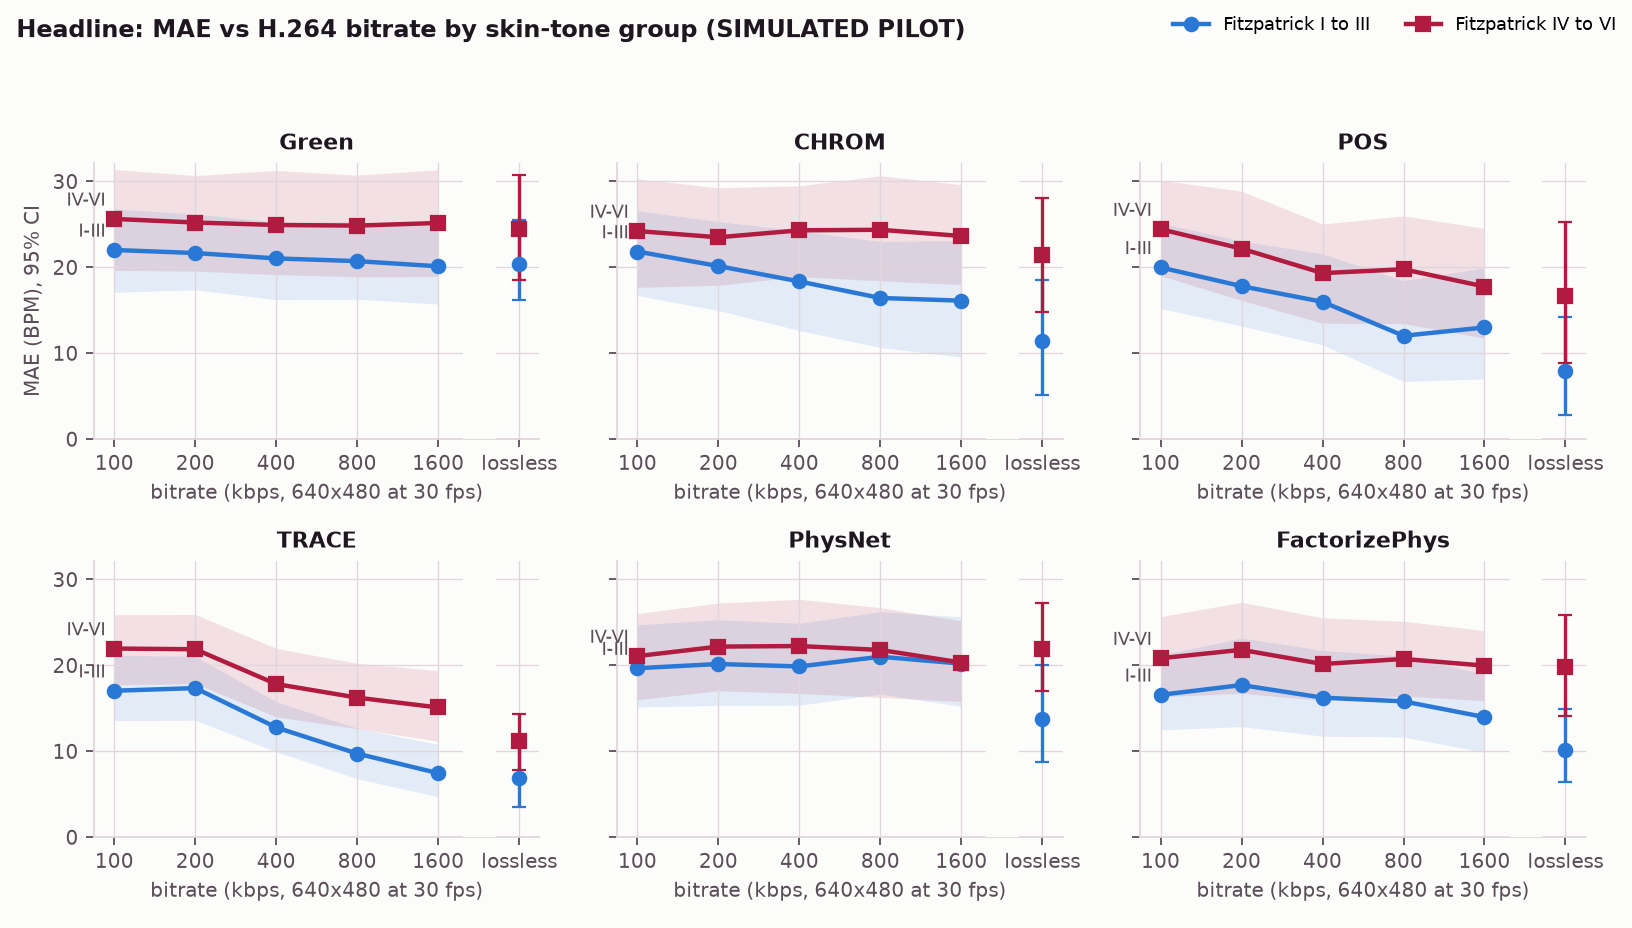
\includegraphics[width=\linewidth]{figures/fan_h264.png}
\caption{MAE against H.264 bitrate for lighter (I to III) and darker (IV to VI) simulated skin. Lossless at right.}
\label{fig:fan}
\end{figure}

Fig.~\ref{fig:fan} shows the headline grid. {{VERDICT_POS}} For CHROM: {{VERDICT_CHROM}} On a still face, the correlation of the decoded skin trace with the true pulse fell from {{FID_LL_II}} (lighter) and {{FID_LL_VI}} (darker) on lossless video to {{FID_100_II}} and {{FID_100_VI}} at 100 kbps H.264.

\textbf{Mitigation.} {{MITIGATION}} On a separate held-out uncompressed cohort, POS scored {{FUSION_POS}} BPM, POS with the artifact mask alone {{FUSION_MASK}}, and TRACE {{FUSION_V2}}; readings TRACE marked confident ({{FUSION_COVERAGE}}\% of windows) had {{FUSION_CONF_MAE}} BPM error against {{FUSION_FLAG_MAE}} for flagged ones.

\textbf{Learned baselines.} PhysNet and FactorizePhys (rPPG-Toolbox \cite{liu2023}, trained on PURE): {{VERDICT_FACTORIZEPHYS}}

\section{Limitations and Next Steps}
Skin-tone physics is modelled, so the simulated result is evidence about the mechanism, not about people. The next step is recording Fitzpatrick III to VI volunteers in Dhaka losslessly with a pulse oximeter; the pilot's variance components give {{POWER_N}} participants per group for 80\% power at {{POWER_EFFECT}} BPM per doubling. Heart-rate variability outputs are wellness indicators, not diagnoses.

\begin{thebibliography}{9}
\bibitem{dasari2021} A. Dasari, S. K. A. Prakash, L. A. Jeni, C. S. Tucker, ``Evaluation of biases in remote photoplethysmography methods,'' \emph{npj Digit. Med.}, 4:91, 2021.
\bibitem{nowara2020} E. M. Nowara, D. McDuff, A. Veeraraghavan, ``A meta-analysis of the impact of skin tone and gender on non-contact photoplethysmography measurements,'' CVPR Workshops, 2020.
\bibitem{mcduff2017} D. McDuff, E. B. Blackford, J. R. Estepp, ``The impact of video compression on remote cardiac pulse measurement using imaging photoplethysmography,'' IEEE FG, 2017.
\bibitem{nowara2019} E. M. Nowara, D. McDuff, ``Combating the impact of video compression on non-contact vital sign measurement using supervised learning,'' ICCV Workshops, 2019.
\bibitem{dehaan2013} G. de Haan, V. Jeanne, ``Robust pulse rate from chrominance-based rPPG,'' \emph{IEEE Trans. Biomed. Eng.}, 60(10), 2013.
\bibitem{wang2017} W. Wang, A. C. den Brinker, S. Stuijk, G. de Haan, ``Algorithmic principles of remote PPG,'' \emph{IEEE Trans. Biomed. Eng.}, 64(7), 2017.
\bibitem{liu2023} X. Liu et al., ``rPPG-Toolbox: Deep remote PPG toolbox,'' NeurIPS Datasets and Benchmarks, 2023.
\end{thebibliography}

\end{document}
